\section{Reconstruction}
\label{sec:Reconstruction}
The reconstruction process is illustrated in figure~\ref{fig:DataFlow} for both real and simulated data.

\begin{figure}[tbh]
  \begin{center}
    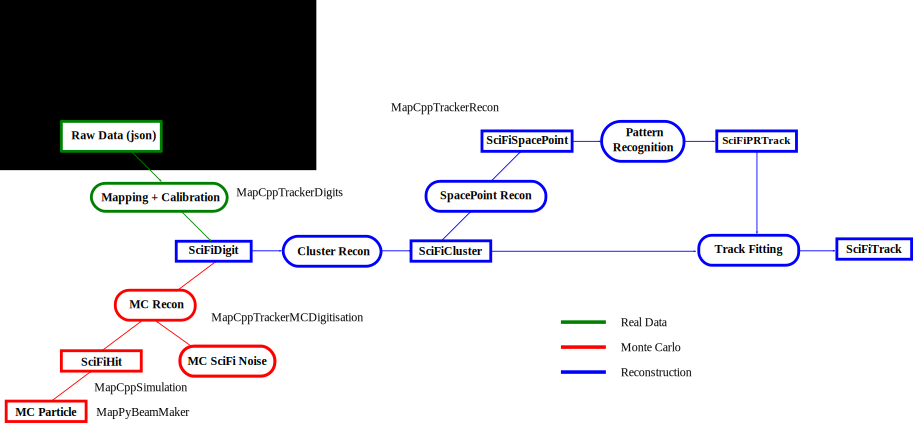
\includegraphics[width=0.95\linewidth]{07-Reconstruction/DataFlow2014.pdf}
    \caption{\label{fig:DataFlow} The reconstruction data flow. Data originates either from simulated or real data, the two branches meet after Digitisation, after which the reconstruction proceeds identically for both.  The relevant MAUS modules for each step are indicated.}
  \end{center}
\end{figure}

  \subsection{Digitization}
  \label{subsec:Digitization}
  For real data the electronic signals produced by the VLPCs are Digitised using analogue-to-Digital converters (ADCs). The DAQ system records the pulse height for each DAQ channel.  Channel-by-channel cailbration constants are used to convert the ADC value to a signal in units of photo-electrons (PE) and the VLPC channel number to tracker channel number.  This information is then used to form a Digit.  The analagous process for Monte Carlo data is described in section~\ref{sec:Simulation}.

  \subsection{Clustering}
  \label{subsec:Clustering}
  A particle that traverses a plane will generate a hit in one or at most two adjacent channels.  An isolated hit or hits in two adjacent channels form a Cluster.  
  
  The Clustering algorithm loops over every combination of pairs of Digits in a SciFiEvent and combines any that occur in neighbouring channels in the same plane. In the case of multi-Digit Cluster, the average channel value is used. The Cluster positioning is defined by the coordinates $(\alpha, \beta)$ where $\alpha$ and the direction of $\beta$ have been defined in Section ~\ref{subsec:PlaneAndClusters}. In the case of two overlapping active channels the value for $\beta$ is determined by solving:
  
  \begin{equation}
    \begin{pmatrix}
     \alpha_1 \\ \beta_1
    \end{pmatrix} = R_{1}^{-1} R_2
    \begin{pmatrix}
      \alpha_2 \\ \beta_2
    \end{pmatrix}
  \end{equation}
  
  \noindent
  where $R_1$, $R_2$ are the rotation matrices that correspond to the orientation of the specified plane. 

  \subsection{Spacepoint Reconstruction}
  \label{subsec:SpacepointReconstruction}
  For each station the constituent planes are searched for Clusters which can be used to define a Spacepoint. Spacepoints are defined by Clusters from all three planes (a triplet Spacepoint) or for any two out of the three planes (a doublet Spacepoint). 
  From the Cluster coordinates, $(\alpha, \beta)$, the $(x, y)$ coordinates of the Spacepoint are determined by rotating into tracker frame.

  \subsubsection{Cluster selection}
  \label{subsubsec:ClusterSelection}
  In order to determine which Clusters from each plane originate from the same track we follow Kuno's conjecture\cite{MiceTrackers} which states that, for a given triplet Spacepoint, the sum of the channel numbers of each Cluster will be a constant.  So if $n^u$, $n^v$ and $n^w$ are the fibre numbers of the Clusters in $u$, $v$ and $w$ and $n^u_0$, $n^v_0$ and $n^w_0$ are the corresponding central channel numbers. Three Clusters form a space point  if:
  \begin{equation}
    | (n^u + n^v + n^w) - (n^u_0 + n^v_0 + n^w_0) | < K \, .
  \end{equation}
  where $K$ is a constant, take by default as 3.0.
  
  Once all triplet Spacepoints have been found, doublet Spacepoints are created from pairs of remaining Clusters. 

  % \subsubsection{Crossing Point Calculation}
  % \label{subsubsec:CrossingPointCalculation}

  \subsection{Pattern Recognition}
  \label{subsec:PatternRecognition}

  Pattern recognition is based on looping over different combinations of Spacepoints and performing a fit using a simple linear least squares technique.  The algorithm treats helical and straight tracks separately, though much of the code is shared. Helical track finding is attempted first then, once all possible helical tracks have been found, any remaining unmatched Spacepoints in the SciFiEvent are passed to the straight line fitting rountines.

   \subsubsection{Helical Pattern Recognition}
   \label{subsubsec:HelicalPatternRecognition}

   The helical pattern recognition is performed in cylindrical co-ordinates $(r, \phi, z)$ where the turning angle $\phi$ defined for $0 \rightarrow \infty$ is distinguished from $\phi '$ the reduced turing angle defined  for $0 \rightarrow 2\pi$. For the helix $s$ is the distance the particle travels measured along the helix. The helix is described by: the circle it describes in the transverse plane $(x_{centre}, y_{centre}, radius)$; $s_0$ the value of $s$ where the helix crosses the reference plane; and $t_s = ds/dz$, which describes the tightness of the coiling. $\phi_0$, the angle of the track as it crosses the tracker reference plane, equivalent to $s_0$, is also used. 

   To find a track one Spacepoint is selected from each station and a circle is fitted in the $(r, \phi')$ projection. If the $\chi^2$ of this fit is sufficiently small (by default less than 15.0 multiplied by the number of degrees of freedom) then the value of $\phi$ is used to generate $s$ and a straight line fit is performed in the $(z,s)$ plane, and if the $\chi^2$ in this projection is also small (by default less than 4.0 multiplied by the number of degrees of freedom) the track is accepted.  $\phi$ itself is determined from $\phi'$ by exploiting the different distances in $z$ between successive tracker stations.  The change in $\phi$ between the hits in any two stations, divided by the distance between those stations, gives a constant which is the same for any pair of hits.  This can then be used to infer the true values of $\phi$.

   All possible combinations of five Spacepoints, one from each station are tested. Points can only be associated with one track. Then all combinations of any remaining Spacepoints are searched, this time requiring Spacepoints from four out of the five stations to form a helix. Tracks with momentum almost parallel to the solenoid axis (i.e. with low transverse momentum, $p_T$) will not suffer an appreciable bend and will not be found by the helix search and so any Spacepoints remaining after the helical tracks have been found are passed to the straight track finding algorithm.

    \subsubsection{Straight Line Pattern Recognition}
    \label{subsubsec:StraightLinePatternRecognition}

    Straight lines are fitted to the Spacepoints when there is no magnetic field and on any Spacepoints remaining after the helix fit is complete. The latter is to identify tracks with a small $p_T$ which are not bent sufficiently in the magnetic field to form a recognisable helix (it has been observed from Monte Carlo studies that the efficiency of the helix finding algorithm begins to tail off for tracks with $p_T < 10 MeV/c$).

    The fit is done in Cartesian coordinates and the track parameters are: $(x_0, y_0, t_x, t_y)$ where $t_x = dx/dz$ and $t_y = dy/dz$. Two Spacepoints are chosen in the outer chambers and a road is created between them. Any Spacepoints in the road are fitted, using Least Sqaures, in the $(x,z)$ and $(y,z)$ planes. The Spacepoints with the lowest $\chi^2$ are chosen as long as their value is less than a predefined cut value (by default less than 15.0 multiplied by the number of degrees of freedom). As in the helical case, following the completion of the full 5 point track search, tracks with Spacepoints in 4 out of the 5 stations are searched for. For the straight case only, following the completetion of the search for 4 point tracks, a search is also made for tracks with Spacepoints in only 3 out of the 5 stations. 

   \subsection{Track Fit}
   \label{subsec:FinalTrackFit}
   The final track fit was implemented using a track-orientated Kalman filter\cite{Fruhwirth,Billoir}, which can be shown to be an optimal linear fitter, that takes into account all correlations and measurements, for a linear system. The Kalman Filter is an iterative algorithm that incrementally propagates an estimate of the current track state between measurement planes, using measurement information to ``filter'' the state, improving the estimate of the track state.
   
   For the helical track fit, the system is only approximately linear, hence an extended Kalman filter was implemented which analytically propagates the track states between measurements, while the covariance matrices are propagated using a first-order linear approximation to the non-linear system.

   Pattern recognition provides a set of Clusters that are associated with a track, which passed the selection criteria, and a parameterisation of that track based on a least squares fit to the points by a helix or a straight line as appropriate. The track parameters calculated from the least squares fit are used to provide the seed for the Kalman fit and the raw Cluster information is used as the measurement data. The flexibility of the Kalman algorithm permits the effects of individual planes (multiple coulomb scattering (MCS) and energy loss), in addition to the material effects of the Helium gas within the tracker, to be accounted for between each measurement point.

     \subsubsection{Kalman Filtering}

     The track is modelled as a discrete state space function of $z$ (the direction of the beam), indicated by the subscript, $k$, where each tracker plane corresponds to a trackpoint and contains a measurement and a track state. Equation~\ref{equ:kalman_system_equation} describes how the true state space vector, $\mathbf{x}_{k,t}$, is assumed to propagate to a subsequent measurement plane. The matrix, $\mathbf{F}_k$, is the Kalman Propagator and describes the first order description of the propagtion between measurement planes. $\mathbf{w}_k$ represents some ``process noise'', which may affect the system between the two measurement planes and is assumed to be gaussian distributed white noise.
    \begin{equation}
      \mathbf{x}_{k,t} = \mathbf{F}_{k-1}\mathbf{x}_{k-1,t} + \mathbf{w}_{k-1}
      \label{equ:kalman_system_equation}
    \end{equation}
    \begin{equation*}
      \textrm{exp}(\mathbf{w}) = 0 \quad\quad \textrm{and} \quad\quad \textrm{cov}(\mathbf{w}) = \mathbf{Q}
    \end{equation*}
     
     The tracker measurements are interpreted in a different state space to the track, allowing measurements of any dimension to be used to filter the track. Equation~\ref{equ:kalman_measurement_equation} describes how the true track state is ``measured'' to be transformed into the measurement space. The matrix, $\mathbf{H}_k$, is the Kalman Measurement Matrix and describes, to first order, the transformation from track state space to the measurement state space. $\mathbf{\varepsilon}_k$ represents some ``measurement noise'' which may smear the measurement of the true state space, it is also assumed to be gaussian distributed.
    \begin{equation}
      \mathbf{m}_k = \mathbf{H}_kx_{k,t} + \mathbf{\varepsilon}_k
      \label{equ:kalman_measurement_equation}
    \end{equation}
    \begin{equation*}
      \textrm{exp}(\mathbf{\varepsilon}) = 0 \quad\quad \textrm{and} \quad\quad \textrm{cov}(\mathbf{\varepsilon}) = \mathbf{V}
    \end{equation*}

    For each measurement plane that contains a measurement, the current estimate for the track state vector is ``filtered'' using the measurement information. This is acheived using the residual between the estimate for the track state and the measurement data, in the measurement state space. Equation~\ref{equ:kalman_state_filtered} describes how the predicted state vector, $\mathbf{x}_{k}^{k-1}$ is filtered using the Kalman Gain Matrix, $\mathbf{K}_k$, to produce the filtered track estimate, $\mathbf{x}_k$. Equation~\ref{equ:kalman_gain_matrix} defines the Kalman Gain Matrix.
    \begin{equation}
      \mathbf{x}_k = \mathbf{x}_k^{k-1} + \mathbf{K}_k ( \mathbf{m}_k - \mathbf{H}_k \mathbf{x}_k^{k-1} )
      \label{equ:kalman_state_filtered}
    \end{equation}
    The predicted covariance matrix, $\mathbf{C}_k^{k-1}$, is filtered in a similar  fashion to produce the filtered covariance matrix, $\mathbf{C}_k^{k}$, as described in equation~\ref{equ:kalman_covariance_filtered}:
    \begin{equation}
      \mathbf{C}_k = ( \mathbf{I} - \mathbf{K}_k \mathbf{H}_k ) \mathbf{C}_k^{k-1}
      \label{equ:kalman_covariance_filtered}
    \end{equation}
    The Kalman Gain matrix is calculated by:
    \begin{equation}
      \mathbf{K}_k = \mathbf{C}_k^{k-1} \mathbf{H}_k^\mathsf{T} (\mathbf{V}_k + \mathbf{H}_k \mathbf{C}_k^{k-1} \mathbf{H}_k^\mathsf{T})^{-1}
      \label{equ:kalman_gain_matrix}
    \end{equation}

    The sequence of prediction and filtering is repeated for all the measurement planes, starting from station~5, plane~2, where the predicted state vector and covariance matrix is determined from the pattern recognition fit parameters, to station~1, plane~0, the reference plane. Once the reference plane has been reached, the state vector will have been sequentially filtered using all the measurements in turn to create the optimal estimate of the track state at that plane. The fit can then be smoothed, whereby the optimal state vector is propagated in reverse down the length of the track, such that all the subsequent measurements can be used to re-adjust previous state vector estimates. This is dsecribed in~\cite{Fruhwirth}


    \subsubsection{The MAUS Kalman Filter Implementation}
    In order to implement a flexible re-usable Kalman Filter, the core algorithm was implemented without any dependencies on phase space dimensions or physical effects. Due to this only the system specific functionality need be provided for a complete implmentation.
    The principal components of the implementation are: propagation routines for both helical and straight tracks; a measurement routine that correctly transforms the track state space into the measurement state space; and approximations for the process and measurement noise.
    
    The measurements correspond to individual Clusters, hence the parameter $\alpha$ (see section~\ref{subsec:PlaneAndClusters}) forms a one-dimensional measurement state. The measurement noise corresponds to the statistical spread of measurements within a single channel in the tracker readout. If the channel is modelled as a top-hat function, the variance of the function is calculated as $w^2/12$, where $w$ corresponds to the width of the channel. Therefore the measurement noise was assumed to be $w/\sqrt{12}$ for all Clusters.

    The process noise was implmented as a combination of MCS and energy straggling. The energy loss  was is calculated using the Landau-Vavilov formula, for the most probable energy loss, and applied during the propagation stage. The noise term itself is calculated per increment, as an RMS scattering angle using an implementation of the Highland formula (equation~\ref{equ:highland_formula}), in a fashion almost identicle to the GEANT4 implementation:
    \begin{equation}
      \theta_{RMS} = \frac{13.6\textrm{MeV/c}}{\beta c p} z \frac{x}{X_0}\left( 1 + 0.038 \ln(\frac{x}{X_0} \right)
      \label{equ:highland_formula}
    \end{equation}
    where $\theta_{RMS}$ is the RMS scattering angle through a finite length of material, $\beta c$, $p$ and $z$ are the velocity, momentum and charge of the particle in question, and $x/X_0$ represents the total path length through the material per radiation length. Although the RMS scattering angle does not form a gaussian distribution, the first order approximation is believed to be sufficient.

%    \subsubsection{Goodness of fit}
%    For each fitted track, a test statistic is computed, which is the $\chi^2$ sum over all the trackpoints. It is calculated by $\chi^2\sum_{k=0}^{k=n}\chi_k^2$ where each chisquared update is given by $\chi_{k}^{2}=\mathbf{r}_{k}^{T}\mathrm{R}_{k}^{-1}\mathbf{r}_{k}$: where $r_{k}$ is the residual computed from the filtered state vector. $r_{k}=\mathbf{m}_{k}-\mathrm{H}_{k}\mathbf{a}_{k}$: where $\mathbf{m}_{k}$ is the $k^{th}$  measured point; $\mathbf{a}_{k}$ is the best Kalman estimate of track state vector at the $k^{th}$ intersection point and $\mathrm{H}_{k}$ is the matrix which projects the state vector of the track into the measurement space. $\mathrm{R}_{k}$ is the covariance matrix of the residuals and is given by  $\mathrm{R}_{k}=\mathrm{V}_{k}-\mathrm{H}_{k}\mathrm{C}_{k}\mathrm{H}_{k}^{T}$ where $\mathrm{V}_{k}$ is the measurement covariance matrix and $\mathrm{C}_{k}$ is the projected variance matrix. This definition of  $\chi^{2}$  takes into account correlations in the measurement predictions and, combined with the number of degrees of freedom of the track fit, is used to generate a {\it p-value} for the track, which we use as a measure of fit quality.


%\begin{equation}
%\chi_{k}^{2}=\mathbf{r}_{k}^{T}\mathrm{R}_{k}^{-1}\mathbf{r}_{k}.
%\end{equation}





  
